\documentclass[9pt, notheorems]{beamer}
\setcounter{tocdepth}{4}
\usepackage[utf8]{inputenc}
\usepackage[T1]{fontenc}
\usepackage{lmodern}
\usepackage{amsmath}
\usepackage{amsthm}
\usepackage{amssymb}
\usepackage{mathrsfs}
\usepackage{amsfonts}
\usepackage{stmaryrd}
\usepackage{xfrac}
\usepackage{dsfont}
\usepackage{fancybox}
\usepackage{fancyref}
\usepackage{multicol}
\usepackage{graphicx}
\usepackage{wrapfig}
\usepackage{textcomp}
\usepackage{mathrsfs}
\usepackage{color}
\usepackage{listings}
\usepackage{tikz-cd}
\usepackage{comment}
\usepackage{caption}
\usepackage{shuffle}
\usepackage{multirow}
\usepackage{appendix}
\usepackage{fdsymbol}
\usepackage{float}
\usepackage{algorithm}
\usepackage[noend]{algpseudocode}
\usepackage{qcircuit}
\usepackage{hyperref}

\newcommand{\HRule}{\rule{\linewidth}{0.5mm}}
\newcommand{\Dyck}[1]{\textsc{Dyck$_{#1}$}}
\newcommand{\FA}[1]{\textsc{FindAny$_{#1}$}}
\newcommand{\FFL}[1]{\textsc{FindFixedLength$_{#1}$}}
\newcommand{\FFP}[1]{\textsc{FindFixedPos$_{#1}$}}
\newcommand{\FALM}[1]{\textsc{FindAtLeftMost$_{#1}$}}
\newcommand{\FARM}[1]{\textsc{FindAtRightMost$_{#1}$}}
\newcommand{\FF}[1]{\textsc{FindFirst$_{#1}$}}
\newcommand{\Null}{\textsc{Null}}

\newcommand{\hered}[1]{\paragraph*{Induction:}{#1}}
\newcommand{\init}[1]{\paragraph*{Initialization:}{#1}}
\newcommand{\IH}[1]{\paragraph*{Induction Hypothesis:}{#1}}
\newcommand{\Conc}[1]{\paragraph*{Conclusion:}{#1}}
\newcommand{\remark}[1]{\paragraph*{Remark:}{#1}}
\newcommand{\observation}[1]{\paragraph*{Observation:}{#1}}
\newcommand{\notation}[1]{\paragraph*{Notation:}{#1}}
\newcommand{\property}[1]{\paragraph*{Property:}{#1}}
\newcommand{\ket}[1]{\ensuremath{|#1\rangle}}
\newcommand{\metersymbol}[1]{\begin{tikzpicture}[scale=#1]
    \draw (.8, 0) arc (0:180:.8);
    \draw[->] (0, 0) -- (1, 1);
\end{tikzpicture}
    }

\renewcommand{\comment}[1]{}
\newcommand\blfootnote[1]{%
    \begingroup
    \renewcommand\thefootnote{}\footnote{#1}%
    \addtocounter{footnote}{-1}%
    \endgroup
}

\theoremstyle{definition}
\newtheorem{definition}{Définition}
\newtheorem{proposition}{Proposition}[definition]

\theoremstyle{plain}
\newtheorem{theorem}{Theorem}[section]
\newtheorem{corollary}{Corollary}[theorem]
\newtheorem{lemma}{Lemma}[theorem]

\theoremstyle{definition}
\newtheorem{conjecture}{Conjecture}[definition]
\newtheorem{cproof}{Proof Corollary}[theorem] 
\newtheorem{lproof}{Proof Lemma}[theorem]
\newtheorem{tproof}{Proof Theorem}[section]

\usetheme{Warsaw}

\title[QQC of bounded height Dyck languages.]{{\huge Complexity of recognizing Dyck languages
of bounded height with quantum query algorithms.}}
\author{Maxime CAUTRÈS}
\institute{Faculty of Computing\\ University of Latvia}
\date{31/08/2022}

\addtobeamertemplate{footline}{\ \insertframenumber/\inserttotalframenumber\ }

\AtBeginSection[]
{
  \begin{frame}
  \frametitle{Sommaire}
  \tableofcontents[currentsection, hideothersubsections]
  \end{frame} 
}

\begin{document}

\begin{frame}
    \titlepage
\end{frame}

\section{Introduction.}


\subsection{Quantum query model and complexity.}

\begin{frame}
    \frametitle{Classical and quantum computers are both made with simple components.}
    \begin{minipage}{.45\textwidth}
        \begin{figure}
            \tikzset{every picture/.style={line width=0.75pt}} %set default line width to 0.75pt        
\centering
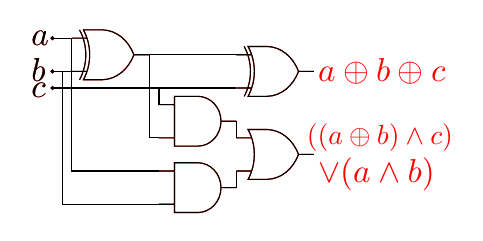
\begin{tikzpicture}[x=0.70pt,y=0.60pt,yscale=-.5,xscale=.5]
    %uncomment if require: \path (0,300); %set diagram left start at 0, and has height of 300

    \visible<1>{
        % Text Node
        \draw[red] (15,48) node [anchor=north west][inner sep=0.75pt]  [xscale=1.2,yscale=1.2] [align=left] {$a$};
        % Text Node
        \draw[red] (15,80) node [anchor=north west][inner sep=0.75pt]  [xscale=1.2,yscale=1.2] [align=left] {$b$};
        % Text Node
        \draw[red] (15,110) node [anchor=north west][inner sep=0.75pt]  [xscale=1.2,yscale=1.2] [align=left] {$c$};

        \filldraw[red] (40, 60) circle (1pt);
        \filldraw[red] (40, 100) circle (1pt);
        \filldraw[red] (40, 120) circle (1pt);
    }
    \visible<2->{
        % Text Node
        \draw (15,48) node [anchor=north west][inner sep=0.75pt]  [xscale=1.2,yscale=1.2] [align=left] {$a$};
        % Text Node
        \draw (15,80) node [anchor=north west][inner sep=0.75pt]  [xscale=1.2,yscale=1.2] [align=left] {$b$};
        % Text Node
        \draw (15,110) node [anchor=north west][inner sep=0.75pt]  [xscale=1.2,yscale=1.2] [align=left] {$c$};

        \filldraw (40, 60) circle (1pt);
        \filldraw (40, 100) circle (1pt);
        \filldraw (40, 120) circle (1pt);
    }

    \visible<2>{
        %Shape: Xor Gate [id:dp7586863585025112] 
        \draw[red]   (72,50) -- (92,50) .. controls (105.95,50.54) and (118.42,62.23) .. (124,80) .. controls (118.42,97.77) and (105.95,109.46) .. (92,110) -- (72,110) .. controls (80.57,91.44) and (80.57,68.56) .. (72,50) -- cycle (60,60) -- (76,60) (60,100) -- (76,100) (124,80) -- (140,80) (68,50) .. controls (76.57,68.56) and (76.57,91.44) .. (68,110) ;
        %Shape: Xor Gate [id:dp4857055310285392] 
        \draw[red]   (242,70) -- (262,70) .. controls (275.95,70.54) and (288.42,82.23) .. (294,100) .. controls (288.42,117.77) and (275.95,129.46) .. (262,130) -- (242,130) .. controls (250.57,111.44) and (250.57,88.56) .. (242,70) -- cycle (230,80) -- (246,80) (230,120) -- (246,120) (294,100) -- (310,100) (238,70) .. controls (246.57,88.56) and (246.57,111.44) .. (238,130) ;
        %Shape: And Gate [id:dp40243073644089766] 
        \draw[red]   (166,130) -- (190,130) .. controls (203.25,130) and (214,143.44) .. (214,160) .. controls (214,176.56) and (203.25,190) .. (190,190) -- (166,190) -- (166,130) -- cycle (150,140) -- (166,140) (150,180) -- (166,180) (214,160) -- (230,160) ;
        %Shape: And Gate [id:dp08349658070673471] 
        \draw[red]   (166,210) -- (190,210) .. controls (203.25,210) and (214,223.44) .. (214,240) .. controls (214,256.56) and (203.25,270) .. (190,270) -- (166,270) -- (166,210) -- cycle (150,220) -- (166,220) (150,260) -- (166,260) (214,240) -- (230,240) ;
        %Shape: Or Gate [id:dp5052546687696813] 
        \draw[red]   (242,170) -- (262,170) .. controls (275.95,170.54) and (288.42,182.23) .. (294,200) .. controls (288.42,217.77) and (275.95,229.46) .. (262,230) -- (242,230) .. controls (250.57,211.44) and (250.57,188.56) .. (242,170) -- cycle (230,180) -- (246,180) (230,220) -- (246,220) (294,200) -- (310,200) ;
    }
    \visible<3->{
        %Shape: Xor Gate [id:dp7586863585025112] 
        \draw   (72,50) -- (92,50) .. controls (105.95,50.54) and (118.42,62.23) .. (124,80) .. controls (118.42,97.77) and (105.95,109.46) .. (92,110) -- (72,110) .. controls (80.57,91.44) and (80.57,68.56) .. (72,50) -- cycle (60,60) -- (76,60) (60,100) -- (76,100) (124,80) -- (140,80) (68,50) .. controls (76.57,68.56) and (76.57,91.44) .. (68,110) ;
        %Shape: Xor Gate [id:dp4857055310285392] 
        \draw   (242,70) -- (262,70) .. controls (275.95,70.54) and (288.42,82.23) .. (294,100) .. controls (288.42,117.77) and (275.95,129.46) .. (262,130) -- (242,130) .. controls (250.57,111.44) and (250.57,88.56) .. (242,70) -- cycle (230,80) -- (246,80) (230,120) -- (246,120) (294,100) -- (310,100) (238,70) .. controls (246.57,88.56) and (246.57,111.44) .. (238,130) ;
        %Shape: And Gate [id:dp40243073644089766] 
        \draw   (166,130) -- (190,130) .. controls (203.25,130) and (214,143.44) .. (214,160) .. controls (214,176.56) and (203.25,190) .. (190,190) -- (166,190) -- (166,130) -- cycle (150,140) -- (166,140) (150,180) -- (166,180) (214,160) -- (230,160) ;
        %Shape: And Gate [id:dp08349658070673471] 
        \draw   (166,210) -- (190,210) .. controls (203.25,210) and (214,223.44) .. (214,240) .. controls (214,256.56) and (203.25,270) .. (190,270) -- (166,270) -- (166,210) -- cycle (150,220) -- (166,220) (150,260) -- (166,260) (214,240) -- (230,240) ;
        %Shape: Or Gate [id:dp5052546687696813] 
        \draw   (242,170) -- (262,170) .. controls (275.95,170.54) and (288.42,182.23) .. (294,200) .. controls (288.42,217.77) and (275.95,229.46) .. (262,230) -- (242,230) .. controls (250.57,211.44) and (250.57,188.56) .. (242,170) -- cycle (230,180) -- (246,180) (230,220) -- (246,220) (294,200) -- (310,200) ;
    }
    \visible<3>{
        %Straight Lines [id:da47322578625017586] 
        \draw[red]    (40,60) -- (60,60) ;
        %Straight Lines [id:da9794654949941013] 
        \draw[red]    (230,160) -- (230,180) ;
        %Straight Lines [id:da4846849793546657] 
        \draw[red]    (230,220) -- (230,240) ;
        %Straight Lines [id:da5854134933106738] 
        \draw[red]    (140,80) -- (140,120) -- (140,180) ;
        %Straight Lines [id:da21543002534508293] 
        \draw[red]    (150,180) -- (140,180) ;
        %Straight Lines [id:da2647954495406195] 
        \draw[red]    (40,120) -- (140.33,120) -- (230,120) ;
        %Straight Lines [id:da3173932178858232] 
        \draw[red]    (40,100) -- (60,100) ;
        %Straight Lines [id:da4191196124425738] 
        \draw[red]    (150,120) -- (150,140) ;
        %Straight Lines [id:da7200697769419422] 
        \draw[red]    (60,60) -- (60,220) -- (150,220) ;
        %Straight Lines [id:da6864505677890691] 
        \draw[red]    (50,100) -- (50,260) -- (150,260) ;
        %Straight Lines [id:da27064207791990746] 
        \draw[red]    (139.67,80) -- (140,80) -- (239.67,80) ;}
    \visible<4->{
        %Straight Lines [id:da47322578625017586] 
        \draw    (40,60) -- (60,60) ;
        %Straight Lines [id:da9794654949941013] 
        \draw    (230,160) -- (230,180) ;
        %Straight Lines [id:da4846849793546657] 
        \draw    (230,220) -- (230,240) ;
        %Straight Lines [id:da5854134933106738] 
        \draw    (140,80) -- (140,120) -- (140,180) ;
        %Straight Lines [id:da21543002534508293] 
        \draw    (150,180) -- (140,180) ;
        %Straight Lines [id:da2647954495406195] 
        \draw    (40,120) -- (140.33,120) -- (230,120) ;
        %Straight Lines [id:da3173932178858232] 
        \draw    (40,100) -- (60,100) ;
        %Straight Lines [id:da4191196124425738] 
        \draw    (150,120) -- (150,140) ;
        %Straight Lines [id:da7200697769419422] 
        \draw    (60,60) -- (60,220) -- (150,220) ;
        %Straight Lines [id:da6864505677890691] 
        \draw    (50,100) -- (50,260) -- (150,260) ;
        %Straight Lines [id:da27064207791990746] 
        \draw    (139.67,80) -- (140,80) -- (239.67,80) ;}

    \visible<4->{
        % Text Node
        \draw[red] (311,80) node [anchor=north west][inner sep=0.75pt]  [xscale=1.2,yscale=1.2] [align=left] {$a\oplus b\oplus c$};
        % Text Node
        \draw[red] (300,160) node [anchor=north west][inner sep=0.75pt]  [xscale=1,yscale=1] [align=left] {$(( a\oplus b) \land c)$};
        % Text Node
        \draw[red] (311,200) node [anchor=north west][inner sep=0.75pt]  [xscale=1.2,yscale=1.2] [align=left] {$ \lor ( a\land b)$};
    }


\end{tikzpicture}
            \caption{A Boolean circuit (Full adder).}
        \end{figure}
    \end{minipage}
    \hfill
    \begin{minipage}{.45\textwidth}
        \begin{figure}
            \vspace*{.5cm}
            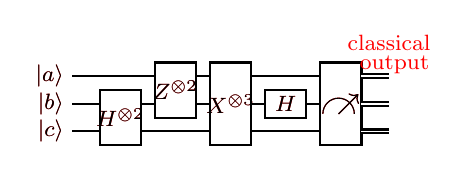
\begin{tikzpicture}[scale=.35]
    \footnotesize
    \visible<1>{
        \draw[red] (-1, 2.5) node[left] {$\ket{a}$};
        \draw[red] (-1, 1.5) node[left] {$\ket{b}$};
        \draw[red] (-1, .5) node[left] {$\ket{c}$};}

    \visible<2->{
        \draw (-1, 2.5) node[left] {$\ket{a}$};
        \draw (-1, 1.5) node[left] {$\ket{b}$};
        \draw (-1, .5) node[left] {$\ket{c}$};}


    \visible<2>{
        \draw[red, thick] (0,0) -- (1.5, 0) -- (1.5, 2) -- (0, 2) -- cycle;
        \draw[thick, red] (2+0,0+1) -- (2+1.5, 0+1) -- (2+1.5, 2+1) -- (2+0, 2+1) -- cycle;
        \draw[thick,red] (4+0,0) -- (4+1.5, 0) -- (4+1.5, 3) -- (4+0, 3) -- cycle;
        \draw[thick,red] (6,0+1) -- (6, 2) -- (7.5, 2) -- (7.5, 1) -- cycle;
        \draw[thick,red] (8+0,0) -- (8+1.5, 0) -- (8+1.5, 3) -- (8+0, 3) -- cycle;
        \draw[red] (.75, 1) node {$H^{\otimes2}$};
        \draw[red] (2.75, 2) node {$Z^{\otimes2}$};
        \draw[red] (4.75, 1.5) node {$X^{\otimes3}$};
        \draw[red] (6.75, 1.5) node {$H$};
        \draw[red] (8.75, 1.5) node {$\metersymbol{.25}$};}

    \visible<3->{
        \draw[thick] (0,0) -- (1.5, 0) -- (1.5, 2) -- (0, 2) -- cycle;
        \draw[thick] (2+0,0+1) -- (2+1.5, 0+1) -- (2+1.5, 2+1) -- (2+0, 2+1) -- cycle;
        \draw[thick] (4+0,0) -- (4+1.5, 0) -- (4+1.5, 3) -- (4+0, 3) -- cycle;
        \draw[thick] (6,0+1) -- (6, 2) -- (7.5, 2) -- (7.5, 1) -- cycle;
        \draw[thick] (8+0,0) -- (8+1.5, 0) -- (8+1.5, 3) -- (8+0, 3) -- cycle;
        \draw (.75, 1) node {$H^{\otimes2}$};
        \draw (2.75, 2) node {$Z^{\otimes2}$};
        \draw (4.75, 1.5) node {$X^{\otimes3}$};
        \draw (6.75, 1.5) node {$H$};
        \draw (8.75, 1.5) node {$\metersymbol{.25}$};}

    \visible<3>{

        \draw[red,thick] (-1, .5) -- (0, .5);
        \draw[red,thick] (1.5, .5) -- (4, .5);
        \draw[red,thick] (5.5, .5) -- (8, .5);
        \draw[red,thick, double] (9.5, .5) -- (10.5, 0.5);


        \draw[red,thick] (-1, 1.5) -- (0, 1.5);
        \draw[red,thick] (1.5, 1.5) -- (2, 1.5);
        \draw[red,thick] (3.5, 1.5) -- (4, 1.5);
        \draw[red,thick] (5.5, 1.5) -- (6, 1.5);
        \draw[red,thick] (7.5, 1.5) -- (8, 1.5);
        \draw[red,thick, double] (9.5, 1.5) -- (10.5, 1.5);


        \draw[red,thick] (-1, 2.5) -- (2, 2.5);
        \draw[red,thick] (3.5, 2.5) -- (4, 2.5);
        \draw[red,thick] (5.5, 2.5) -- (8, 2.5);
        \draw[red,thick, double] (9.5, 2.5) -- (10.5, 2.5);}

    \visible<4->{

        \draw[thick] (-1, .5) -- (0, .5);
        \draw[thick] (1.5, .5) -- (4, .5);
        \draw[thick] (5.5, .5) -- (8, .5);
        \draw[thick, double] (9.5, .5) -- (10.5, 0.5);


        \draw[thick] (-1, 1.5) -- (0, 1.5);
        \draw[thick] (1.5, 1.5) -- (2, 1.5);
        \draw[thick] (3.5, 1.5) -- (4, 1.5);
        \draw[thick] (5.5, 1.5) -- (6, 1.5);
        \draw[thick] (7.5, 1.5) -- (8, 1.5);
        \draw[thick, double] (9.5, 1.5) -- (10.5, 1.5);


        \draw[thick] (-1, 2.5) -- (2, 2.5);
        \draw[thick] (3.5, 2.5) -- (4, 2.5);
        \draw[thick] (5.5, 2.5) -- (8, 2.5);
        \draw[thick, double] (9.5, 2.5) -- (10.5, 2.5);}

    \visible<4>{
        \draw[red] (10.5, 3.7) node {classical};
        \draw[red] (10.7, 2.9) node {output};}

\end{tikzpicture}\\[.8cm]
            \caption{A Quantum circuit.}
        \end{figure}
    \end{minipage}
\end{frame}

\begin{frame}
    \frametitle{Interacting with qubits is more more complexe.}

    \begin{minipage}{.45\textwidth}
        \visible<1->{
            \begin{figure}
                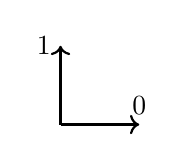
\begin{tikzpicture}
                    \draw[thick, ->] (0, 0) -- (1, 0);
                    \draw[thick, ->] (0, 0) -- (0, 1);
                    \draw (1, 0) node[above] {0};
                    \draw (0, 1) node[left] {1};
                \end{tikzpicture}
                \caption{A classical bit}
            \end{figure}}
        \visible<3->{
            \begin{figure}
                \begin{tabular}{c|c||c}
                    $A$ & $B$ & $A\oplus B$ \\
                    \hline
                    0   & 0   & 0           \\
                    0   & 1   & 1           \\
                    1   & 0   & 1           \\
                    1   & 1   & 0           \\
                \end{tabular}
                \caption{Truth table on 2 bits.}
            \end{figure}}
    \end{minipage}
    \hfill
    \begin{minipage}{.45\textwidth}
        \visible<2->{
            \begin{figure}
                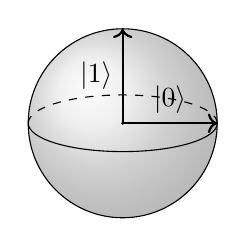
\begin{tikzpicture}[scale=.6]
                    \shade[ball color = gray!40, opacity = 0.4] (0,0) circle (2cm);
                    \draw (0,0) circle (2cm);
                    \draw (-2,0) arc (180:360:2 and 0.6);
                    \draw[dashed] (2,0) arc (0:180:2 and 0.6);
                    \fill[fill=black] (0,0) circle (1pt);
                    \draw[thick, ->] (0,0 ) -- node[above]{$\ket{0}$} (2,0);
                    \draw[thick, ->] (0,0) -- node[left]{$\ket{1}$} (0, 2);
                \end{tikzpicture}
                \caption{A quantum bit.}
            \end{figure}}
        \visible<4->{
            \begin{figure}
                $H^{\oplus2} =\frac{1}{2}
                    \begin{bmatrix}
                        1 & 1  & 1  & 1  \\
                        1 & -1 & 1  & -1 \\
                        1 & 1  & -1 & -1 \\
                        1 & -1 & -1 & 1
                    \end{bmatrix}$
                \caption{Unitary matrix on 2 qubits.}
            \end{figure}}
    \end{minipage}
\end{frame}

\begin{frame}
    \frametitle{Quantum query algorithm is just a quantum circuit.}
    \begin{figure}[h!]
        \centering
        $
            \Qcircuit @C=.8em @R=1em {
            \lstick{\vdots} & \qw & \multigate{2}{U_0}  & \multigate{2}{Q} & \multigate{2}{U_1} & \qw &  & &  \multigate{2}{Q} & \multigate{2}{U_T}&\multigate{2}{\metersymbol{.2}} & \cw\\
            &\lstick{\ket{\psi_{start}}} qw & \ghost{U_0} & \ghost{Q} & \ghost{U_1} & \qw & \cdots & & \ghost{Q} & \ghost{U_T} & \ghost{\metersymbol{.2}}& \cw\\
            \lstick{\vdots}& \qw & \ghost{U_0} & \ghost{Q}  & \ghost{U_1} & \qw & & &\ghost{Q} &\ghost{U_T}&\ghost{\metersymbol{.2}}& \cw \\
            }$
        \caption{Structure of a quantum query algorithm.}
        \label{fig:quantum_query_algorithm_structure}
    \end{figure}
\end{frame}

\subsection{Dyck languages of bounded height}

\begin{frame}
    \frametitle{Dyck words}
\end{frame}

\begin{frame}
    \frametitle{Dyck word of bounded hight}
\end{frame}

\subsection{History of the problem}

\begin{frame}
    \frametitle{The trichotomy article}
\end{frame}

\begin{frame}
    \frametitle{There is two main direction of study}

\end{frame}

\begin{frame}
    \frametitle{Goal of the internship}
\end{frame}

\section{State of the art}

\subsection{Lower bounds to the QQC of \Dyck{k,n}}

\begin{frame}
    \frametitle{Dont speak to muck abour it}
    \begin{itemize}
        \item \textbf{By reduction:}
        \item \textbf{By adversary method:}
    \end{itemize}
    MOre information in the report
\end{frame}

\subsection{Upper bounds to the QQC of \Dyck{k,n}}

\begin{frame}
    \frametitle{Algorithms gives QQC upper bounds.}
\end{frame}

\begin{frame}
    \frametitle{Reduction to transmit the QQC upper bounds .}

\end{frame}

\section{The progress to reduce the \Dyck{k,n} QQC .}

\subsection{Why does the problem is not only a grover search }

\begin{frame}
    \frametitle{FOr k >=2 it is not more easy}



\end{frame}

\subsection{Original algorithm and small revisions }

\begin{frame}
    \frametitle{presentation of the algorithm}



\end{frame}

\begin{frame}
    \frametitle{small revision}



\end{frame}

\subsection{A new algorithm for k=2}

\begin{frame}
    \frametitle{the new algorithm}



\end{frame}

\begin{frame}
    \frametitle{can be plug in the big one}



\end{frame}

\section{New idea to get better quantum query complexity bounds }

\subsection{lower bounds: try to do reduction from other problem}
\begin{frame}
    \frametitle{}



\end{frame}
\subsection{Upper bounds: Trying not do to every node}
\begin{frame}
    \frametitle{}



\end{frame}
\subsection{Conclusion}

\begin{frame}
    \frametitle{Conclusion}
    \textbf{What as been done:}
    \begin{itemize}
        \item
    \end{itemize}
    \textbf{Possible idea to go further:}
    \begin{itemize}
        \item
    \end{itemize}

\end{frame}

\end{document}
